\documentclass[12pt]{article}
\usepackage{amsmath}
\usepackage{amssymb}
\usepackage{geometry}
\usepackage{enumerate}
\usepackage{natbib}
\usepackage{float}%稳定图片位置
\usepackage{graphicx}%画图
\usepackage[english]{babel}
\usepackage{a4wide}
\usepackage{indentfirst}%缩进
\usepackage{enumerate}%加序号
\usepackage{multirow}%合并行
\usepackage[colorlinks,linkcolor=red]{hyperref}
\title{\large UM-SJTU JOINT INSTITUTE\\Technology Entrepreneurship\\(VX425)\\\ \\\ \\\ \\\ \\\ \\\ \\\ \\\ \\\ \\\ \\\
Individual Report\\\ \\\ Social Entrepreneurship Business Model Canvas \\\ \\\ \\\ \\\ \\\ \\\ \\\ }
\author{Name: Pan Chongdan\\ID: 516370910121}
\date{Date: \today}

\begin{document}
\maketitle
\newpage
\section{Characteristics of Social Entrepreneurship }
Social entrepreneurship is a special kind of entrepreneurship focusing more on social welfare rather than profits so it a has different business model according to its distinctions:
\begin{enumerate}
\item \textbf{Creativity} includes goal setting and problem-solving, which enable social entrepreneurs to know what they want to happen and how to achieve success.
\item \textbf{Entrepreneurs quality} enables entrepreneurs to have vision of how society will be different when their idea is at work, and they can't stop until that their idea is at work across the whole society.
\item \textbf{Social impact} measures the idea's intrinsic worth and its ability to change the society even without its founder.
\item \textbf{Ethical fiber} describes the entrepreneur's motivation. It's social objectives that inspire them to compete in marketplace with other competitors.
\end{enumerate}  
\section{Business Model for Social Entrepreneurship}
Business model canvas for common entrepreneurship has 9 blocks, however it's different for social entrepreneurship due to its own characteristics.
\begin{figure}[H]
\centering
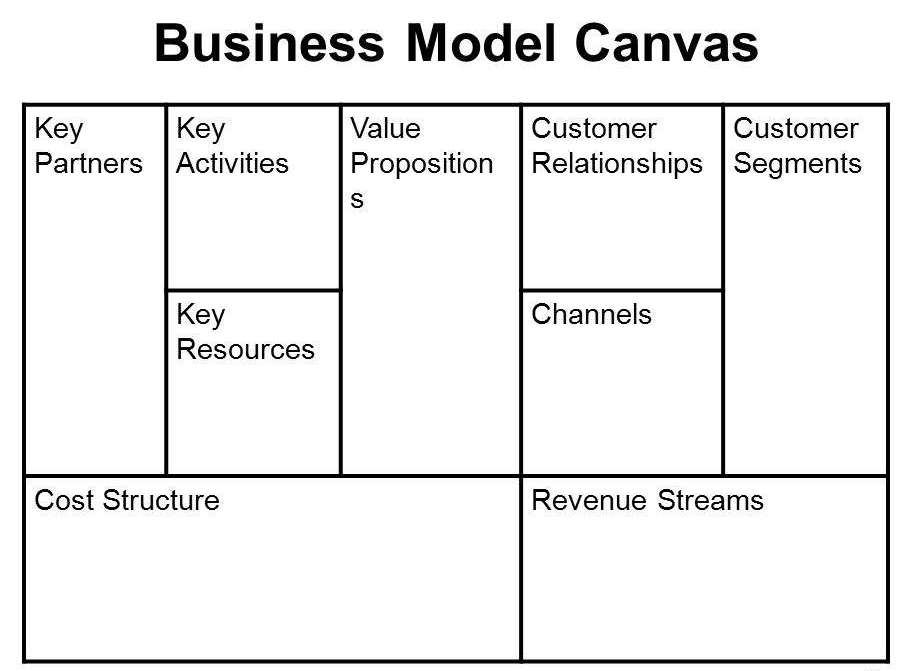
\includegraphics[scale=0.2]{P1.png}
\caption{Common business model canvas}
\end{figure}
\par For social entrepreneurship, the customers are less important, while social objectives and the area which the business focused on is necessary for the model. Hence, in my model, there is no customer relationships, channels and customer segments but social objectives and business domain are added.
\begin{figure}[H]
\centering
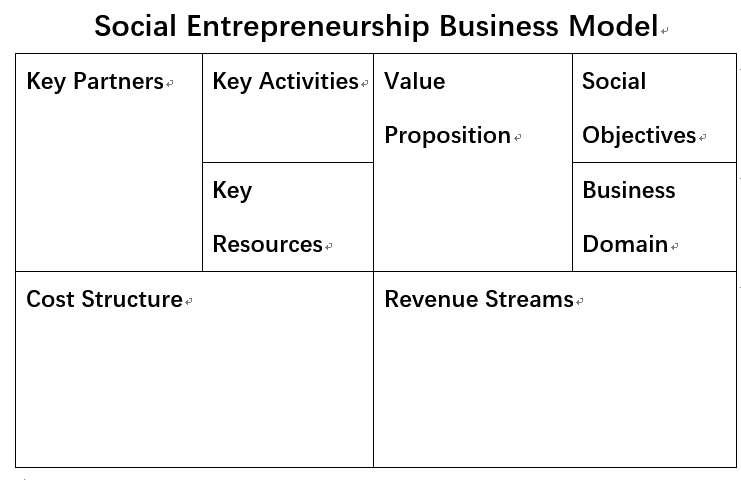
\includegraphics[scale=0.4]{P2.png}
\caption{Business model canvas for social entrepreneurship}
\end{figure}
\subsection{Value Proposition}
Social entrepreneurship has value proposition but usually it aims at bringing more social impact rather than profit. Value proposition is the foundation of a social entrepreneurship and it shows the entrepreneur's creativity and entrepreneurship quality. Social entrepreneurship usually provides service or products promoting its value proposition which can have a far-reaching impact on the society. 
\subsection{Social Objective}
Social objective is one of the most important and distinctive parts of social entrepreneurship's business model because it describes how society will be affected by the value promoted by the business's product or service. It can also reflect the entrepreneurship's ethical fiber and motivation.
\subsection{Business Domains}
Social entrepreneurship not necessarily has customer segment because it want to affect the total society. However, social entrepreneurship must has some business domain to focus on, which can be a group of people or some field based on the social objective. For instance, for a business focuses on environment protection there is no customer segment but its business domain is environment and culture.
\subsection{Key Activities}
Key activities is important for social entrepreneurship because business must make social impact with such activities. For example, on of key activities for poverty relief is infrastructure construction.
\subsection{Customer Relationships and Channels}
Since there is no typical customers for social entrepreneurship, then customer relationships and channels are not essential in the model. Furthermore, even though sometimes there are some target audience for the social entrepreneurship, they are probably social disadvantaged group and need help from social entrepreneurship without various channels. 
\subsection{Key Resources and Key Partners}
Social entrepreneurship needs key resources and key partners to reach their social objective. Since social entrepreneurship tends to have effects on a wide range of people, so it needs approval from government to ensure the outcomes are positive. In this case, government is the key partner and its approval is a sort of resources.
\subsection{Cost structure and Revenue Streams}
Even social entrepreneurship doesn't focus too much on making profit, it still needs revenue streams to cover costs and maintain operation, otherwise the entrepreneurship can't develop sustainability.
\section{Case Study}
\subsection{International Committee of the Red Cross}
International Committee of the Red Cross is a social entrepreneurship founded by Swiss citizen in 1863, aiming at do works during wars, helping sufferers from war and spread humanitarianism. Of course, ICRC has its business model canvas for social entrepreneurship.
\begin{enumerate}[-]
\item The \textbf{value proposition} is to provide medical and mental help for victims of wars and protect them from war and injuries.
\item Their \textbf{social objective} is to spread humanitarianism among the world and advocate peace. Their social objective has influenced the society a lot. On May.8th, which is World Red Cross and Red Crescent Day, many people will promote education and knowledge related the theme decided by ICRC.
\item The \textbf{business domain} for ICRC covers various area, including health, restoring family links, access to education etc. 
\begin{figure}[H]
\centering
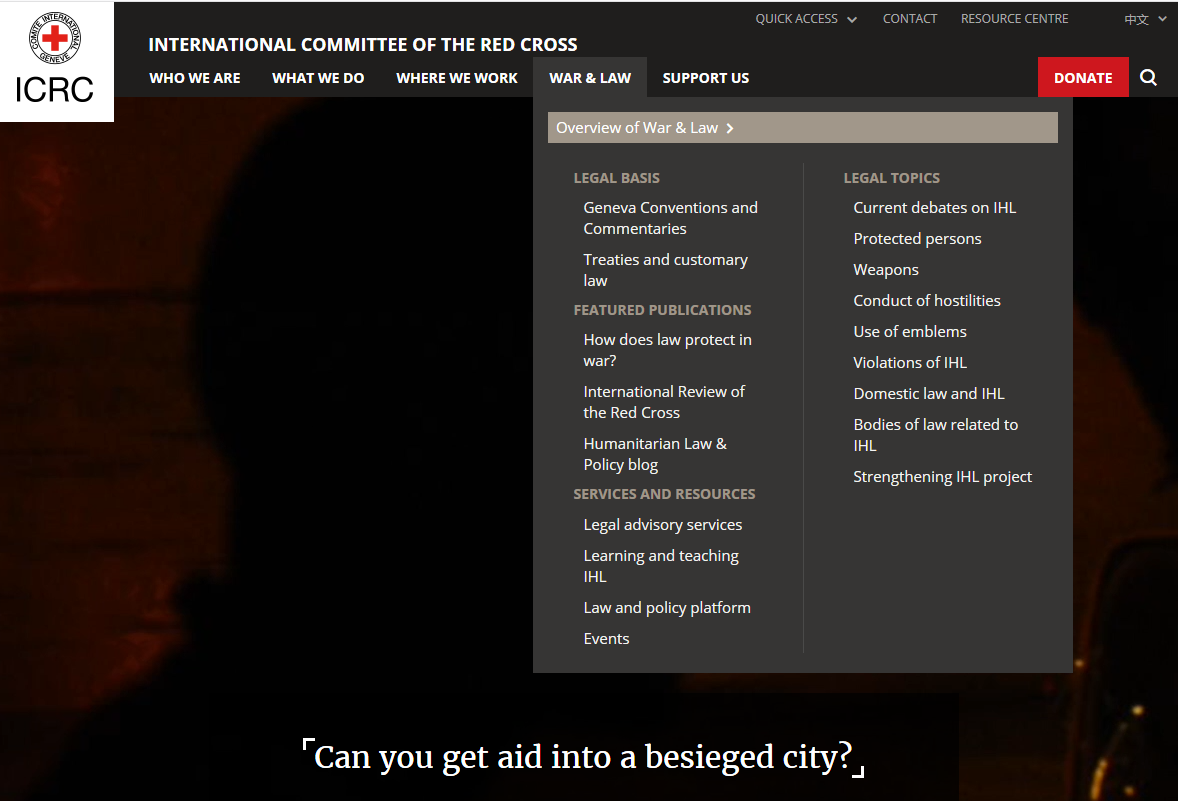
\includegraphics[scale=0.25]{P3.png}
\end{figure}
From the official website of ICRC, we can see most important and primary area for ICRC is war.
\item
ICRC's \textbf{key activities} are various, all of which aims at promoting its value proposition and make enough social impact. For example, ICRC dispatches works to teach first-aid knowledge for the public. When there is a war, many ICRC's workers will go to the front and treat casualties of war.
\begin{figure}[H]
\centering

\includegraphics[scale=0.4]{P4.png}
\caption{ICRC's various activities}
\end{figure} 
\item The \textbf{key resources} of ICRC mainly includes money and volunteers. Since ICRC is a social entrepreneurship, all money are used to cover budget while volunteers devoted themselves into delivering aid for victims directly.
\item The \textbf{key partners} of ICRC are united nation, army, governments and corporations. In time of war, army will provide ICRC with access to war zone and protect them. No army will attack ICRC volunteers even though they're helping the enemy. In addition, government and corporations help ICRC to develop and manufacture devices used in key activities. 
\item 
\begin{figure}[H]
\centering
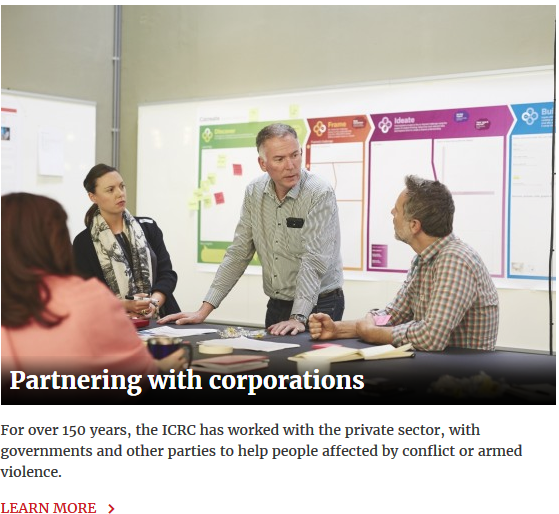
\includegraphics[scale=0.4]{P5.png}
\end{figure}
ICRC's \textbf{revenue streams} mainly come from donation provided by governments, supranational organization and public and private resources. Governments are the main donor covering 84.1\% of last five year's budget.
\begin{figure}[H]
\centering
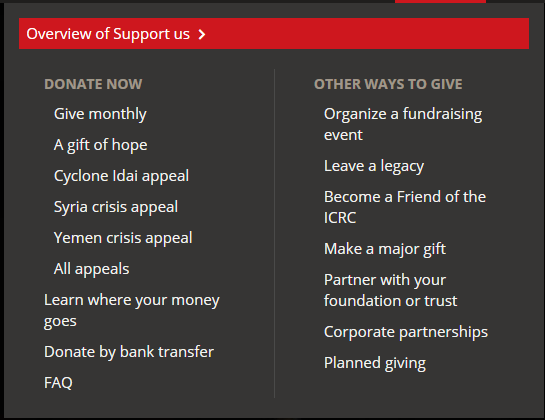
\includegraphics[scale=0.4]{P6.png}
\caption{ICRC's revenue stream}
\end{figure}
\item ICRC's budget for \textbf{cost structure} is quite huge, reaching over 2 billion in 2019 with 3.9\%. The cost structure have 3 parts: the humanitarian needs of the communities affected, the ability to deliver aid and protection to those communities, and a realistic assessment of what can actually be implemented. 
\end{enumerate}
\section{Conclusion}
In conclusion, the business model for social entrepreneurship focuses on the society and is based on social entrepreneurship's characteristics.
\begin{figure}[H]
\centering
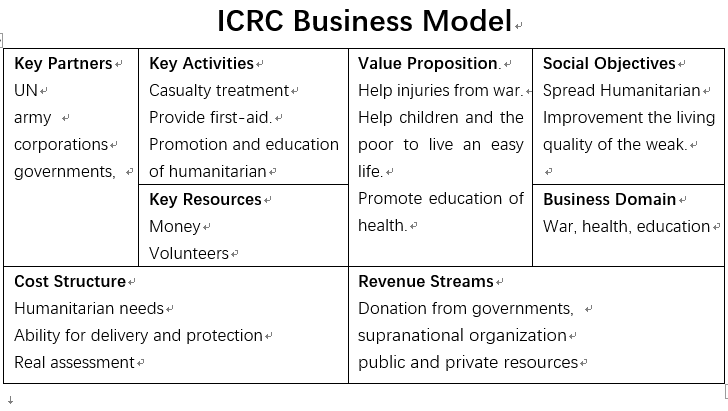
\includegraphics[scale=0.5]{P7.png}
\caption{ICRC business model}
\end{figure}
ICRC is one of the most representative social entrepreneurship and its model can also be applied on others.
\section{Bibliography}
\begin{enumerate}
\item Bornstein, David. \emph{How to Change the World}. New York: Oxford University Press. pp. 
\item \url{https://wiki.mbalib.com/wiki/Social_entrepreneurship}
\item \url{http://slideplayer.com/slide/5905106/}
\item \url{https://wenku.baidu.com/view/8e384c61854769eae009581b6bd97f192379bf08.html}
\item \url{http://www.sohu.com/a/123676996_114819}
\item \url{https://www.icrc.org/zh/contact/}
\item \url{https://www.icrc.org/}

\end{enumerate}
\end{document}